%\documentclass[dvipdfmx,fleqn]{beamer}
\documentclass[dvipdfmx,fleqn,handout]{beamer}
\usepackage{amsmath,amssymb,amsthm}

\mode<presentation>
{
  \usetheme{default}
}
\title{\Large Fictitious Play 発表資料}
\author{\large 大野 嵩侃}
\date{\small 2014年6月28日}

\usefonttheme{professionalfonts}

\setbeamercovered{transparent=20}

\setbeamertemplate{navigation symbols}{} 
\setbeamertemplate{footline}[frame number] 



\begin{document}

\sffamily
\gtfamily


\begin{frame}
  \titlepage
  \thispagestyle{empty}
\end{frame}

\setcounter{framenumber}{0}




\begin{frame}
\frametitle{目次}
\begin{itemize}\setlength{\parskip}{0.5em}
\item
Fictitious Playの説明
\item
コードの説明
\item
プログラムを用いたFictitious Playのシミュレーション 
\begin{itemize}\setlength{\parskip}{0.5em}
 \item
 Matching Pennies Game
 \item
 Coordination Game
 \end{itemize}
\item
まとめ
\end{itemize}
\end{frame}



\begin{frame}
\frametitle{一般的なFictitious Playの説明}
\begin{itemize}\setlength{\parskip}{0.5em}
\item
一定の利得表のもとで、プレイヤー0,プレイヤー1の2人が標準型ゲームを複数回繰り返す\pause
\item
プレイヤーはそれぞれ「相手はこのような確率分布で行動する」という信念をもち、その確率分布の下で自らの期待利得が最大となるような行動をとると仮定する\pause
\item
ある期における信念が、その期以前に相手が実際にとった行動の経験分布と一致する場合に、この動学モデルを\emph{Fictitious Play}とよぶ\pause
\item
今回は厳密なそれとは少し異なるが、同様に相手の行動の経験分布が信念に大きな影響を与えるモデルを考えた
\end{itemize}
\end{frame}


\begin{frame}
\frametitle{今回取り上げるFictitious Playの説明}
\begin{itemize}\setlength{\parskip}{0.5em}
\item
プレイヤーは共に行動0,行動1という2つの選択肢をもつ\pause
\item
$t$回目のゲームを行う直前の時点での確率分布に関する信念のうち、とくにプレイヤー$i$の「相手はこのような確率で行動1をとる」という信念を$x_i(t)$として表すことにする\pause
\item
ゲームを1回も行っていない$t=0$での信念は初期信念$x_i(0)$として$[0,1]$間の一様分布からランダムに定まる\pause
\item
また、$t$期におけるプレイヤー$i$の行動を$a_i(t)$と表すことにする. たとえば
\begin{itemize}\setlength{\parskip}{0.5em}
\item$t=5$でプレイヤー0が行動1をとったら$a_0(5)=1$
\item$t=8$でプレイヤー1が行動0をとったら$a_1(8)=0$
\end{itemize}
\end{itemize}
\end{frame}

\begin{frame}
\frametitle{今回取り上げるFictitious Playの説明}
\begin{itemize}\setlength{\parskip}{0.5em}
\item
$0$期から$k-1$期までのゲームを終えた時点での信念$x_i(k)$は
\[
x_i(k)=\frac{x_i(0)+\sum_{j=0}^{(k-1)} a_{(1-i)}(j)}{k+1}
\]
と表される\\
(初期信念が後の信念に影響する点が通常のfictitious playとは異なる)\pause
\item
たとえば$x_0(0)=0.5$で、$t=0$から$t=8$までの9回でプレイヤー1が7回行動1を選択していたとしたら
$t=9$時点のプレイヤー0の信念$x_0(9)$は以下のようになる
\[
x_0(9)=\frac{0.5+7}{1+9}=\frac{7.5}{10}=0.75
\]
\end{itemize}
\end{frame}

\begin{frame}
\frametitle{今回取り上げるFictitious Playの説明}
\begin{itemize}\setlength{\parskip}{0.5em}
\item
すると、
\[
x_i(k+1)=x_i(k)\times\frac{k+1}{k+2}+a_{(1-i)}(k)\times\frac{1}{k+2}
\]
が成り立つことがわかる\pause
\item
このことから、$x_0(t)$を再帰的に
\[
x_0(t+1)
= x_0(t) + \frac{1}{t+2} (a_1(t) - x_0(t))
\]
と書き表すことができる\pause
\item
上式より、直前の行動が信念に与える影響は次第に小さくなっていくため、各人の信念はいずれ何らかの値に収束してゆくのではないか、と考えられる。\pause
\item
次ページ以降ではこの$2\times2$のfictitious playを表現したプログラムのコードを書き、実際にいくつかのゲームの利得表を代入してプログラムを実行してみることで、この仮説が正しいかを検証したい。
\end{itemize}
\end{frame}

\begin{frame}[fragile]   %[containsverbatim]% verbatim 環境を使えるように
\frametitle{コードの説明}
\begin{itemize}\setlength{\parskip}{0.5em}

\item
プログラムに入れた機能は次の4つである\pause
\item
$n$回のゲームを行い, $t=0,1,\dots,n-1$における$x_i(t)$の推移をプロットした$t-x$グラフを表示する\pause
\item
上記のグラフをPNG,PDF形式で保存する\pause
\item
$n$回のゲームからなるfictitious playを$m$回行い, $x_0(n-1)$がとった値の度数分布をヒストグラムとして表示する\pause
\item
上記のヒストグラムをPNG,PDF形式で保存する\pause
\item
次ページ以降でコードの説明を行う\pause
\item
なお、インデントについては一部割愛しているので注意
\end{itemize}
\end{frame}

\begin{frame}[fragile]   %[containsverbatim]% verbatim 環境を使えるように
\frametitle{インポート}
\begin{itemize}\setlength{\parskip}{0.5em}

\item
\footnotesize
\begin{verbatim}
import matplotlib.pyplot as plt
import random
import numpy as np
\end{verbatim}
\pause
\normalsize
\item
ライブラリのインポートを行う\pause
\begin{itemize}\setlength{\parskip}{0.5em}
\item
matplotlib.pyplotはグラフのプロットに使用 \pause

\item
randomは初期信念と行動を定めるのに使用 \pause

\item
numpyは行列計算に使用
\end{itemize}

\end{itemize}
\end{frame}

\begin{frame}[fragile]% verbatim 環境を使えるように
\frametitle{FPクラスとinitメソッド(1/2)}
\begin{itemize}\setlength{\parskip}{0.5em}
\item

\footnotesize
\begin{verbatim}
class FP:

    def __init__(self, profits):
        self.pro = profits
        self.cu_xs = [0, 0]
        self.x0s = []
        self.x1s = []
 \end{verbatim}\pause
\normalsize

\item
いくつかのメソッドをもつクラスをFPとして定義した\pause\\
FPを使う際には\verb|f = FP(profits)|のように打つ必要がある\pause
\item
\verb|profits|は利得表を表す行列である\\
詳細は次ページで述べる\pause
\item
initメソッド中でインスタンス変数をいくつか定義している\pause\\
これはクラス内の各メソッド中で共有される



\end{itemize}
\end{frame}


\begin{frame}[fragile]% verbatim 環境を使えるように
\frametitle{FPクラスとinitメソッド(2/2)}
\begin{itemize}\setlength{\parskip}{0.5em}
\item

\footnotesize
\begin{verbatim}
class FP:

    def __init__(self, profits):
        self.pro = profits
        self.cu_xs = [0, 0]
        self.x0s = []
        self.x1s = []
 \end{verbatim}\pause
\normalsize
\item
インスタンス変数の説明\pause
\begin{itemize}\setlength{\parskip}{0.5em}

\item
\verb|self.pro|は\verb|profits|と同じであり、たとえば利得行列
\footnotesize
\begin{equation*}
\begin{pmatrix}
(a,b) & (c,d)\\
(e,f) & (g,h)
\end{pmatrix}
\end{equation*}
\normalsize
は
\verb|[[[a,b],[c,d]],[[e,f],[g,h]]]|で表す
\pause
\item
\verb|self.cu_xs|は現在の$(x_0,x_1)$を表すリスト\pause
\item
\verb|self.x0s, self.x1s|は$t=0,1,2,\dots$での$x_0,x_1$をそれぞれ左から並べたリスト

\end{itemize}

\end{itemize}
\end{frame}



\begin{frame}[fragile]% verbatim 環境を使えるように
\frametitle{oneplayメソッド(1/5)}
\begin{itemize}\setlength{\parskip}{0.5em}
\item

\footnotesize
\begin{verbatim}
def oneplay(self, ts_length):
       pro_cal = (np.transpose(self.pro)[0],
                  np.transpose(np.transpose(self.pro)[1]))
       self.x0s = []
       self.x1s = []
       self.cu_xs = [random.uniform(0, 1), random.uniform(0, 1)]
       cu_es = [[0, 0], [0, 0]]
 \end{verbatim}\pause
\normalsize

\item
\verb|oneplay|は\verb|ts_length|の値の回数だけゲームを行い、$x_0(t),x_1(t)$の値の推移を記録するメソッド\pause\\
最初に\verb|x0s, x1s|を空にすることでこのoneplayを複数回行えるようにしている\\
(これがないと何回も繰り返した時に要素が無尽蔵に増える)\pause
\item
\verb|pro_cal|に関しては次ページで詳しく述べる
\item
\verb|cu_xs|はランダムに定まる初期信念$x_0(0),x_1(0)$の値になる\pause
\item
\verb|cu_es|はその時点で各プレイヤーが各行動をとったときの期待利得を表し、ここではリストの形だけを定めている
\end{itemize}
\end{frame}


\begin{frame}[fragile]% verbatim 環境を使えるように
\frametitle{oneplayメソッド(2/5)}
\begin{itemize}\setlength{\parskip}{0.5em}
\item
\footnotesize
\begin{verbatim}
def oneplay(self, ts_length):
    pro_cal = (np.transpose(np.transpose(self.pro)[0]),
                    np.transpose(self.pro)[1])
       self.x0s = []
       self.x1s = []
       self.cu_xs = [random.uniform(0, 1), random.uniform(0, 1)]
       cu_es = [[0, 0], [0, 0]]
 \end{verbatim}
\normalsize
\item
\verb|pro_cal|は利得表をそのまま書き写したのに近い\verb|profits|を計算しやすいよう転置を用いて書き換えたもの\pause
\footnotesize
\begin{equation*}
\begin{pmatrix}
(a,b) & (c,d)\\
(e,f) & (g,h)
\end{pmatrix}
\end{equation*}
\normalsize
を表すリスト\verb|[[[a,b],[c,d]],[[e,f],[g,h]]]|に対してこの操作を行うと\pause
\verb|[array[[a,c],[e,g]],array[[b,f],[d,h]]|となる。\\すなわち
\footnotesize
\begin{equation*}
\begin{pmatrix}
a & c\\
e & g
\end{pmatrix},
\begin{pmatrix}
b & f\\
d & h
\end{pmatrix}
\end{equation*}
\normalsize
という形に変形される
\item
\end{itemize}
\end{frame}
 
\begin{frame}[fragile]% verbatim 環境を使えるように
\frametitle{oneplayメソッド(3/5)}
\begin{itemize}\setlength{\parskip}{0.5em}
\item
\footnotesize
\begin{verbatim}   
for i in range(ts_length):
    self.x0s.append(self.cu_xs[0])
    self.x1s.append(self.cu_xs[1])
    exp = ((1-self.cu_xs[0], self.cu_xs[0]),
           (1-self.cu_xs[1], self.cu_xs[1]))
    cu_es[0] = np.dot(pro_cal[0], exp[0])
    cu_es[1] = np.dot(pro_cal[1], exp[1])
    cu_as = [0, 0]
\end{verbatim}\pause
\normalsize
\item
1回毎のゲームを\verb|ts_length|の回数繰り返す\pause
\item
まず\verb|x0s|に\verb|cu_xs[0]|,\verb|x1s|に\verb|cu_xs[1]|を加えている\pause
\\n回これを繰り返すと$t=0,1,\dots,n-1$における$x_0(t),x_1(t)$の値がそれぞれ順番に記録される
\item
\verb|exp|はプレイヤー2人が考える相手の行動の確率分布を行列の形で表したもの\pause\\
いま、\verb|cu_xs|は[$x_0(t),x_1(t)$]となっているので、\verb|exp|は以下のようになる\pause
\footnotesize
\begin{equation*}
\begin{pmatrix}
1-x_0(t) & x_0(t)\\
1-x_1(t) & x_1(t)
\end{pmatrix}
\end{equation*}
\normalsize
\end{itemize}
\end{frame}

\begin{frame}[fragile]% verbatim 環境を使えるように
\frametitle{oneplayメソッド(4/5)}
\begin{itemize}\setlength{\parskip}{0.5em}
\item
\footnotesize
\begin{verbatim}   
(for i in range(ts_length):)
     cu_es[0] = np.dot(pro_cal[0], exp[0])
     cu_es[1] = np.dot(pro_cal[1], exp[1])
     cu_as = [0, 0]
\end{verbatim}\pause
\normalsize
\item
期待利得を表す\verb|cu_es|の値を計算する\pause\\
\verb|np.dot|は行列の積を表すので、ここでやっている計算は
\footnotesize
\begin{equation*}
\begin{pmatrix}
a & c\\
e & g
\end{pmatrix}\cdot
\begin{pmatrix}
1-x_0(t) \\
x_0(t)
\end{pmatrix}
, 
\begin{pmatrix}
b & f\\
d & h
\end{pmatrix}\cdot
\begin{pmatrix}
1-x_1(t)\\
x_1(t)
\end{pmatrix}
\end{equation*}
\normalsize
の2つである\pause
\item
\verb|cu_as|はある時点での実際の行動を表すリストで、ここでは形だけを定めている
\end{itemize}
\end{frame}


\begin{frame}[fragile]% verbatim 環境を使えるように
\frametitle{oneplayメソッド(5/5)}
\begin{itemize}\setlength{\parskip}{0.5em}
\item
\footnotesize
\begin{verbatim}
(for i in range(ts_length):)
     for j in range(2):
         if cu_es[j][0] == cu_es[j][1]:
             cu_as[j] = random.randint(0, 1)
         else:
             cu_as[j] = cu_es[j].argmax()
     for k in range(2):
         self.cu_xs[k] = (self.cu_xs[k]*(i+1)+cu_as[1-k])/(i+2)
\end{verbatim}\pause
\normalsize
\item
\verb|for j|以下で両プレイヤーの行動を定める
 \begin{itemize}\setlength{\parskip}{0.5em}\pause
 \item
行動0と行動1の期待利得が同じならランダムに定める\pause
 \item
異なる場合は\verb|argmax()|によって期待利得が大きい方の行動を選択する\pause\\
たとえば\verb|cu_xs[0] = [3,-2]|の場合に\verb|argmax()|を使うと最大値3のリスト内の順番である0が返ってくる\pause
\end{itemize}
\item
\verb|for k|以下で信念をアップデートする
\begin{itemize}\setlength{\parskip}{0.5em}
\item
計算はFictitious Playの説明通り
\end{itemize}
\end{itemize}
\end{frame}

\begin{frame}[fragile]% verbatim 環境を使えるように
\frametitle{playplotメソッド(1/2)}
\begin{itemize}\setlength{\parskip}{0.5em}
\item
\footnotesize
\begin{verbatim}
def playplot(self, ts_length):
    self.oneplay(ts_length)
    plt.plot(self.x0s, 'b-', label='x_0(t)')
    plt.plot(self.x1s, 'r-', label='x_1(t)')
    plt.legend()
    plt.show()
\end{verbatim}
\normalsize
\pause
\item
\verb|oneplay|メソッドを実行して記録された$x_0(t),x_1(t)$の推移をプロットするメソッド\pause
\item
\verb|playplot(1000)|のように入力すると実行される\pause\\
この場合は$t=0,1,\dots,999$について記録されている\pause
\item
たとえば次のような利得行列でこのメソッドを実行する
\footnotesize
\begin{equation*}
\begin{pmatrix}
(1,-1) & (-1,1)\\
(-1,1) & (1,-1)
\end{pmatrix}
\end{equation*}\pause
\normalsize
すると次ページのようなグラフが得られる
\end{itemize}
\end{frame}

\begin{frame}
\frametitle{playplotメソッド(2/2)}
\begin{figure}
 \centering
 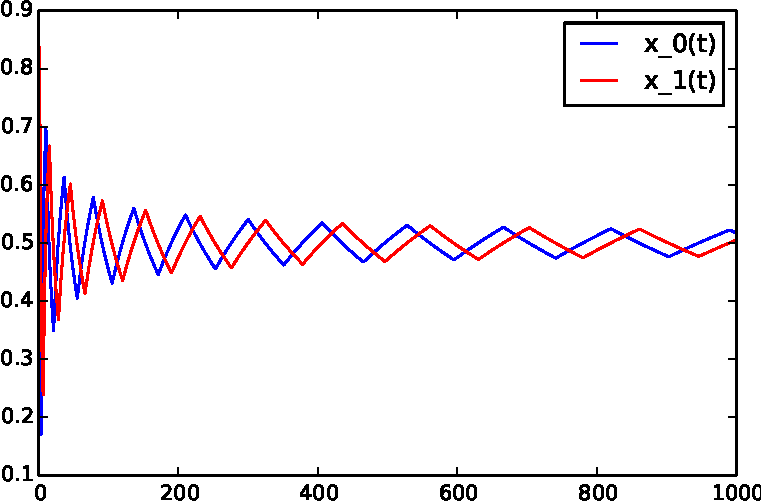
\includegraphics[width=\linewidth]{oneplay2.pdf}
 \label{fig:matchingpennies_plot}
\end{figure}
\end{frame}

\begin{frame}[fragile]% verbatim 環境を使えるように
\frametitle{playsaveメソッド}
\begin{itemize}\setlength{\parskip}{0.5em}
\item
\scriptsize
\begin{verbatim} 
def playsave(self, ts_length, name):
    self.oneplay(ts_length)
    plt.plot(self.x0s, 'b-', label='x_0(t)')
    plt.plot(self.x1s, 'r-', label='x_1(t)')
    plt.legend()
    plt.savefig(str(name)+'.png', bbox_inches='tight', pad_inches=0)
    plt.savefig(str(name)+'.pdf', bbox_inches='tight', pad_inches=0)
    plt.close()
\end{verbatim}
\normalsize
\pause
\item
前ページで表示したグラフを表示することなくPNGとPDFで保存するメソッド\pause
\item
\verb|playsave(1000,'fictplay')|のように入力して実行\pause\\
この場合は$t=0,1,\dots,999$についての推移を表すグラフを"fictplay.png"および"fictplay.pdf"として保存している\pause
\item
保存するグラフを前もって見ることができないため、推移が何種類か考えられるようなものを漏らさず保存するのには不向き\pause\\
\end{itemize}
\end{frame}



\begin{frame}[fragile]% verbatim 環境を使えるように
\frametitle{histogramメソッド(1/2)}
\begin{itemize}\setlength{\parskip}{0.5em}
\item
\footnotesize
\begin{verbatim}
def histogram(self, n, ts_length):
    last_x0s = []
    for j in range(n):
        self.oneplay(ts_length)
        last_x0s.append(self.cu_xs[0])
\end{verbatim}\pause
\normalsize
\item
\verb|oneplay|メソッドを何回も実行し、各回における最終的な$x_0$の値を記録するメソッド
\pause
\item
\verb|histogram(100,1000)|のように入力して実行\pause\\
この場合$x_0(1000)$を100回分記録することになる
\pause
\item
リストである\verb|last.x0s|に記録が行われる\pause\\
\verb|oneplay|が終わるごとにその時点での\verb|cu_xs[0]|が追加される
\end{itemize}
\end{frame}


\begin{frame}[fragile]% verbatim 環境を使えるように
\frametitle{histogramメソッド(2/2)}
\begin{itemize}\setlength{\parskip}{0.5em}
\item
\footnotesize
\begin{verbatim}
ax = plt.subplot(111)
ax.hist(last_x0s, alpha=0.6, bins=5)
ax.set_xlim(xmin=0, xmax=1)
t = 'ts = '+str(ts_length)+', times = '+str(n)
ax.set_title(t)
\end{verbatim}\pause
\normalsize
\pause
\item
\verb|last_x0s|からヒストグラムを作り、表示せずにバックグラウンドでプロットしている
\pause
\item
確率分布としてわかりやすいよう$x$の範囲は0から1まで
\item
\verb|last_x0s|の最大値から最小値を引いた値を5等分したものがヒストグラムの1本1本の幅となる
\end{itemize}
\end{frame}


\begin{frame}[fragile]% verbatim 環境を使えるように
\frametitle{histplotメソッド(1/2)}
\begin{itemize}\setlength{\parskip}{0.5em}
\item
\footnotesize
\begin{verbatim}
def histplot(self, n, ts_length):
    self.histogram(n, ts_length)
    plt.show()
\end{verbatim}
\normalsize
\pause
\item
\verb|histogram|メソッドでバックグラウンドにプロットしたものを表示するメソッド
\item
\verb|histplot(100,1000)|のように入力して実行する\pause\\
このとき表示されるグラフは100回分の$x_0(1000)$の値の度数を表すヒストグラムである
\pause
\\
これによって次ページのようなグラフが表示される
\end{itemize}
\end{frame}

\begin{frame}
\frametitle{histplotメソッド(2/2)}
\begin{figure}
 \centering
 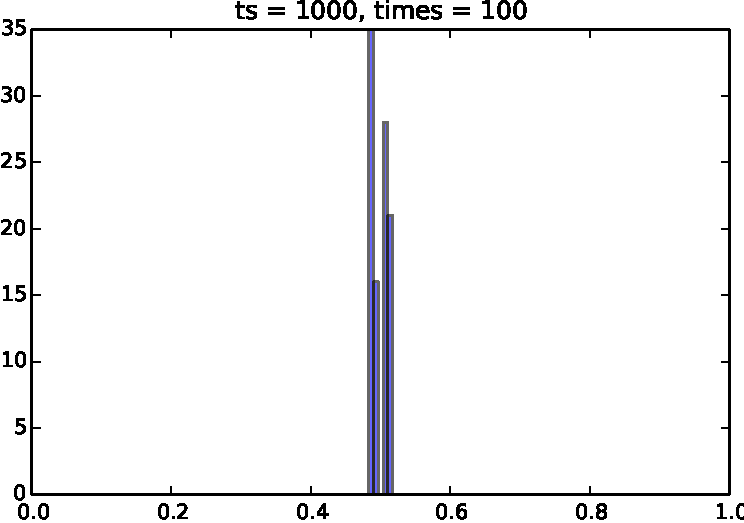
\includegraphics[width=\linewidth]{histogram2.pdf}
 \label{fig:matchingpennies_plot}
\end{figure}
\end{frame}

\begin{frame}[fragile]% verbatim 環境を使えるように
\frametitle{histsaveメソッド}
\begin{itemize}\setlength{\parskip}{0.5em}
\item
\scriptsize
\begin{verbatim}
def histsave(self, n, ts_length, name):
    self.histogram(n, ts_length)
    plt.savefig(str(name)+'.png', bbox_inches='tight', pad_inches=0)
    plt.savefig(str(name)+'.pdf', bbox_inches='tight', pad_inches=0)
    plt.close()
\end{verbatim}
\normalsize
\item
前ページで表示したグラフを表示することなくPNGとPDFで保存するメソッド\pause
\item
\verb|histsave(100,1000,'ficthist')|のように入力して実行\pause\\
この場合は100回分の$x_0(1000)$の値についてのヒストグラムを"ficthist.png"および"ficthist.pdf"として保存している
\end{itemize}
\end{frame}



\begin{frame}
\frametitle{具体的なゲームにおけるプログラムの実行}
\begin{itemize}\setlength{\parskip}{0.5em}
\item
ここまでで説明したコードを用いて、特定の利得表で表されるゲームの様子を実際に求めてみる
\item
今回行うのは次の2つのゲームである\pause
\begin{itemize}\setlength{\parskip}{0.5em}
\item
Matching Pennies Game
\item
Coordination Game
\end{itemize}
\end{itemize}
\end{frame}



\begin{frame}
\frametitle{Matching Pennies}
\begin{itemize}\setlength{\parskip}{0.5em}

\item
Matching Pennies Gameは以下のような利得表をもつ単純なゲームである
 \begin{table}
 \begin{tabular}{|c|c|c|} \hline
      & 行動0 & 行動1 \\ \hline 
    行動0 & 1,-1 & -1,1 \\ \hline
    行動1 & -1,1 & 1,-1 \\ \hline
   \end{tabular}
  \end{table}\pause
\item
このゲームに純粋戦略ナッシュ均衡は存在しない\pause
\item
また、混合戦略ナッシュ均衡は両者ともに$(0.5,0.5)$(のみ)である \pause
\item
このため、$x_i(t)$が収束するのであればそれは$0.5$と予測される\pause
\item
実際にプログラムを実行し、描画したグラフおよびヒストグラムはコードの説明で用いたものに等しい
\item
図より、たしかにこのゲームでのfictitious playでは両者の混合戦略は$(0.5,0.5)$に収束するとわかる

\end{itemize}
\end{frame}

\begin{frame}
\frametitle{Coordination}
\begin{itemize}\setlength{\parskip}{0.5em}
\item
Coordination Gameは以下のような利得表をもつゲームである
 \begin{table}
 \begin{tabular}{|c|c|c|} \hline
    & 行動0 & 行動1 \\ \hline 
    行動0 & 4,4 & 0,3 \\ \hline
    行動1 & 3,0 & 2,2 \\ \hline
   \end{tabular}
  \end{table}\pause
\item
このゲームの純粋戦略ナッシュ均衡は
$(a_1,a_2)=(0,0),(1,1)$
の2つである\pause
\item
また、混合戦略ナッシュ均衡は両者ともに
$(\frac{2}{3},\frac{1}{3})$
のみである
\pause
\item
この3つのナッシュ均衡点への収束が何らかの比率で実現すると考えられるが$\cdots\cdots$?
\item
次ページにcoordination gameで$t=100$のfictitious playを200回行ったヒストグラムを示す
\end{itemize}
\end{frame}

\begin{frame}
\frametitle{Coordination}
\begin{figure}
 \centering
 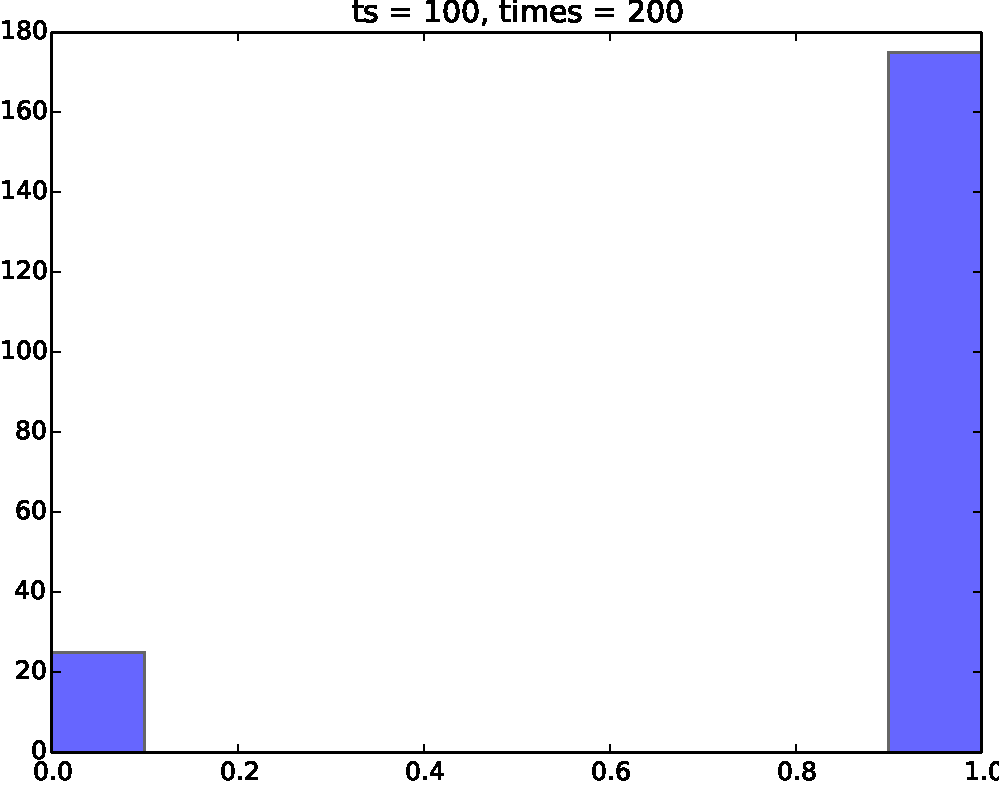
\includegraphics[width=\linewidth]{coordhist.pdf}
 \label{fig:coordination_hist}
\end{figure}
\end{frame}


\begin{frame}
\frametitle{Coordination}
\begin{itemize}\setlength{\parskip}{0.5em}
\item
前ページのヒストグラムより、3つのナッシュ均衡点のうち混合戦略ナッシュ均衡は実現していないことがわかる\pause
\item
これはこのゲームが「相手と同じ戦略を取るのがよい」という性質を持つゲームであり、どちらかの$x_i(t)$が0あるいは1に一定以上近づいた時点でもう片方もその行動を優先するようになるためであると考えられる\pause
\item
$x_i(t)$が1に収束したパターンと0に収束したパターンのグラフを次に記す\pause\\
いずれもmatching penniesに比べ収束が速いことがわかる
\end{itemize}
\end{frame}

\begin{frame}
\frametitle{Coordination}
\begin{figure}
 \centering
 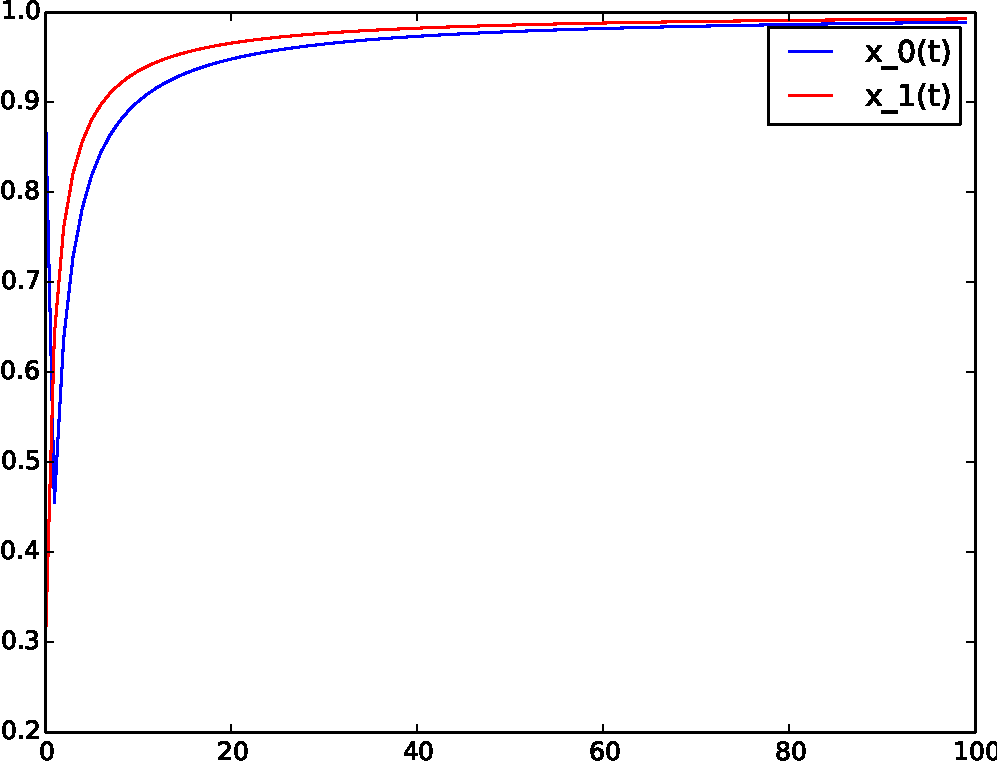
\includegraphics[width=\linewidth]{coordplay0.pdf}
 \label{fig:coordination}
\end{figure}
\end{frame}


\begin{frame}
\frametitle{Coordination}
\begin{figure}
 \centering
 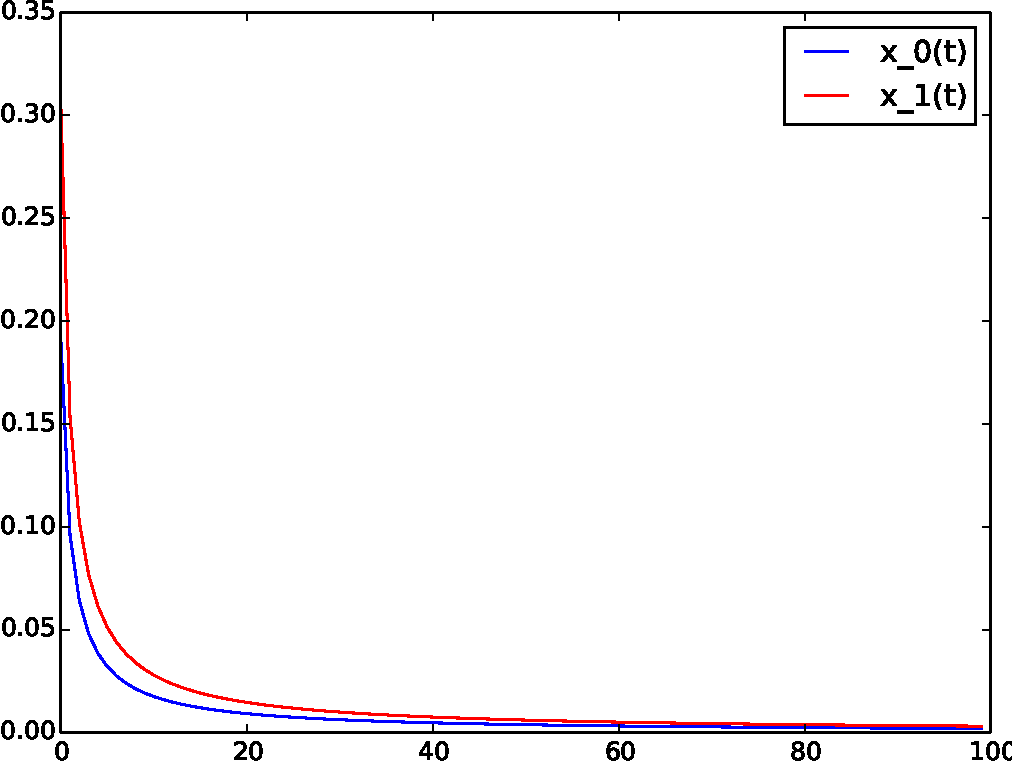
\includegraphics[width=\linewidth]{coordplay1.pdf}
 \label{fig:coordination}
\end{figure}
\end{frame}

\begin{frame}
\frametitle{まとめ}
\begin{itemize}\setlength{\parskip}{0.5em}
\item
fictitious playではナッシュ均衡点に収束してゆく\pause
\item
だが、ナッシュ均衡点の全てが収束先となるわけではない
\end{itemize}
\end{frame}

\begin{frame}
\frametitle{よくわかっていない点・今後の課題}
\begin{itemize}\setlength{\parskip}{0.5em}
\item
coordination gameで混合戦略ナッシュ均衡が実現しないことの証明\pause
\item
np.transpose()を利得行列に使った際に行われている処理\pause\\
おそらく利得行列は3次元配列の行列として扱われている\\
3次元配列での転置とは何をどうしているのか$\cdots\cdots$?
\item
ヒストグラムをプロットする際、現在は値が出た区間を5等分しているが、これを結果にかかわらず$[0,1]$の区間を10等分するように変えたい

\end{itemize}
\end{frame}
\end{document}